As said above, our implementation uses 2 octree layers: one for the scene browsing,
and one for the meshes' browsing. Thats means the algorithm uses nested loops.
\begin{figure}[H]
    \centering
    \begin{lstlisting}[morekeywords={foreach}]
foreach intersected node in the scene octree
{ // loop 1
  foreach mesh in this scene node
  { // loop 2
    foreach intersected node in mesh s octree
    { // loop 3
      foreach triangle in this mesh node
      {
        intersect_triangle();
      }
    }
  }
}
    \end{lstlisting}
    \caption{Octree layers' browsing loops}
    \label{code:octree_layers_loops}
\end{figure}

Therefore, the problem is when we are coming to very detailed meshes, some thread
of a same warp might have less loop~3's iterations in loop~1's first iterations,
but more loop~3's iterations in loop~1's second iterations for instance. But since
there are executed in the same warp, all loop will be synchronized. Meaning all
loop shall finish at the same time. The idea of this optimization
is to collapses loop~1, 2 and 3 as shown on Figure~\ref{code:octree_layers_loops}
by an one loop based state machine.

\begin{figure}[h]
    \centering
    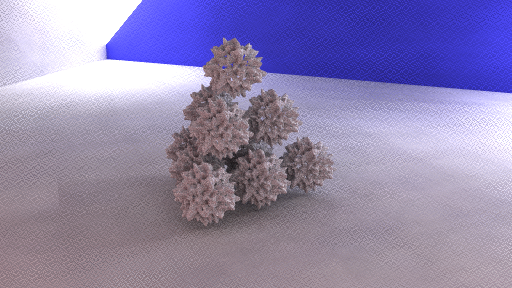
\includegraphics[width=0.8\columnwidth]{render_displaced_spheres.png}
    \caption{Displaced spheres}
    \label{fig:displaced_spheres}
\end{figure}

\begin{figure}[h]
    \centering
    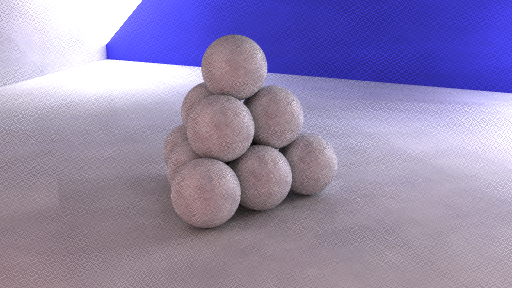
\includegraphics[width=0.8\columnwidth]{render_spheres.png}
    \caption{Simple spheres}
    \label{fig:spheres}
\end{figure}

\begin{figure}[H]
    \tiny
    \centering
    \begin{tabular}{ | l | c | c | }

        \hline
        Octree one loop & Simple spheres & Displaced spheres \\
        \hline
        Disabled & 374.2ns & 1746.9ns \\
        Enabled & 410.1ns & 1522.2ns \\
        \hline

    \end{tabular}
    \caption{Octree one loop browsing's average rendering time per ray}
    \label{table:octree_one_loop_browsing}
\end{figure}

We can actually witness on Figure~\ref{table:octree_one_loop_browsing} that
there is a rendering time improvement on a scene having nearby detailed meshes
(as Figure~\ref{fig:displaced_spheres} shows), thanks to the removal of the warp's thread
synchronisation caused by the nested loops, improving the warp efficiency. But
when rendering scene having non-detailed meshes (as Figure~\ref{fig:spheres} shows), we
are witnessing a performance drop, caused by the states-machine's conditions
overload.
